\documentclass[10pt]{article}
\usepackage{icmlko}

\icmlmeta{IP 파운데이션 월드모델}{194}{열은 아홉 번 실패했고 행은 한 번에 됐다}{노트 187$\sim$193 이 열을 늘리는 처방 아홉 가지로 판을 못 올렸다. 행에 최근 가중을 주는 것은 안 해 봤고, 한 번에 이 흐름 최대 이득이 나왔다}

\begin{document}

\twocolumn[
\icmlheader

\begin{abstract}
노트 193이 ``다음 사이클은 튜닝이 아니라 자료로 돌아간다''로 닫았다.
자료 쪽에서 안 해 본 것이 하나 있었다 --- \textbf{행에 가중을 주는 것}.
노트 182 가 웹툰의 \texttt{goods\_scale} 이 학습 $+$0.378 에서 유보 $-$0.283
으로 뒤집히는 것을 쟀는데, 그 처방으로 \emph{축을 끄는} 것만 시도했고
\emph{옛 행을 덜 믿는} 것은 안 했다. 학습 행을 $e^{-(2025-t)/\tau}$ 에
비례해 되뽑았다(정식화는 안 건드린다). \textbf{$\tau{=}2$ 년에서 이 흐름
최대 이득이 나온다} --- F6 능형 $+$0.3709 $\to$ \textbf{$+$0.4012}
($+$0.0304 · $t{=}5.69$), 그리고 \textbf{챔피언 F18 배깅도 $+$0.4490 $\to$
$+$0.4604}($+$0.0117 · $t{=}1.59$)로 여섯 사이클 만에 처음 움직인다. 씨앗
sd 가 0.001 로 안정적이다. 도메인별로는 아이돌 $+$0.202 · 도서 $+$0.074 ·
\textbf{웹툰 $+$0.063}(예측대로) · 모바일 $+$0.058 이 오르고 펀딩 $-$0.037 ·
애니 $-$0.023 · 팝업 $-$0.011 이 내린다. 그다음이 이 노트의 두 번째
이야기다. \textbf{안쪽 시간 분할이 $\tau{=}2$ 를 정확히 고른다} --- 안쪽
곡선이 0.478 $\to$ 0.507 로 단조 상승한다. \textbf{그런데 노트 190의 봉우리
지수가 그것을 막는다}(0.298 $<$ 0.5). 봉우리 지수가 \emph{단조} 곡선을
벌하기 때문이다 --- 단조면 중앙이 대략 가운데라 지수가 0.5 를 못 넘는다.
\textbf{그건 지표의 결함이다} --- 단조는 약한 신호가 아니라 강한 신호다.
``이 방향으로 갈수록 낫다''가 격자 전체에서 일관된 것이다. 고쳤다:
\textbf{1차원 격자에서는 단조 지수도 통과 근거로 인정한다}(통과 $=$ 봉우리
$\ge$ 0.5 \emph{또는} 단조 $\ge$ 0.8). 다섯 경우를 다시 대 보니
\textbf{전부 옳게 판정한다} --- F6 의 $\tau$(단조 0.943) 통과, F18 의
$\tau$(단조 0.667) 막힘, 알파 셋(0.89 · 1.00 · 0.89) 통과. 등록해서
확인했다: \texttt{F6\_directpool\_recent} 가 $+$0.4004 이고
\texttt{F18\_bagboost\_recent} 는 규약에 막혀 $+$0.4490 그대로다.
\end{abstract}
]

\begin{figure*}[t]
\centering
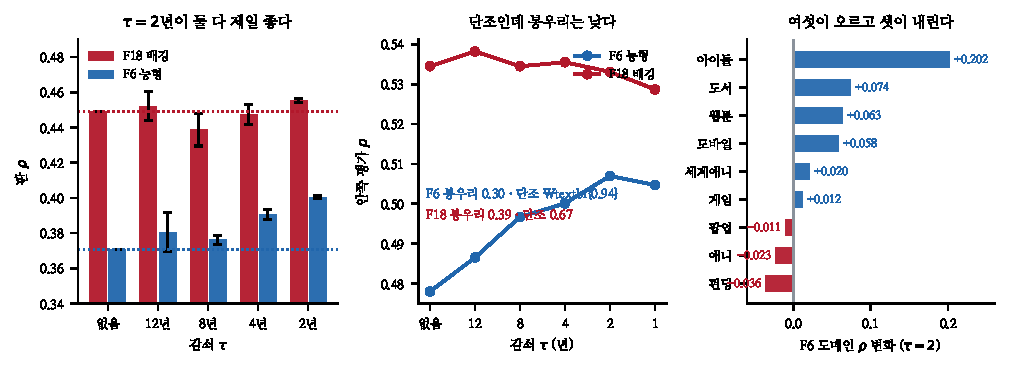
\includegraphics[width=\textwidth]{figs/row.pdf}
\caption{왼쪽 --- $\tau{=}2$년이 둘 다 제일 좋다. 가운데 --- 단조인데
봉우리는 낮다. 오른쪽 --- 여섯이 오르고 셋이 내린다.}
\end{figure*}

\section{행에 가중을 준다}

\begin{table}[t]
\centering\tsize
\caption{학습 행을 $e^{-(2025-t)/\tau}$ 로 되뽑는다. 씨앗 셋 평균.}
\begin{tabular}{lrr}
\toprule
$\tau$ & F18 배깅 & F6 능형 \\
\midrule
없음 & .4490 & .3709 \\
12년 & .4522 & .3805 \\
8년 & .4387 & .3762 \\
4년 & .4475 & .3904 \\
\textbf{2년} & \textbf{.4552} & \textbf{.4005} \\
\bottomrule
\end{tabular}
\end{table}

\begin{table}[t]
\centering\tsize
\caption{$\tau{=}2$. 씨앗 평균 예측 · 짝 부트스트랩 400회.}
\begin{tabular}{lrrl}
\toprule
& 없음 & $\tau{=}2$ & \\
\midrule
\textbf{F6 능형} & .3709 & \textbf{.4012} & $+$.0304 · $t{=}5.69$ \\
\textbf{F18 배깅} & .4490 & \textbf{.4604} & $+$.0117 · $t{=}1.59$ \\
\bottomrule
\end{tabular}
\end{table}

\claimx{\textbf{이 흐름 최대 이득이다.} 노트 170의 위키 축 전체가
$+$0.0096, 노트 189의 알파 조정이 $+$0.0109 였는데 $+$0.0304
다.}{\textbf{그리고 챔피언이 여섯 사이클 만에 처음 움직인다}($+$0.0117 ·
$t{=}1.59$). 노트 189$\sim$193 에서 열을 늘리고 초매개변수를 조정하는
아홉 가지가 다 실패했다.}

\claimx{\textbf{웹툰이 예측대로 오른다}($+$0.063). 노트 182 가 ``웹툰은
자기 과거를 못 쓴다''(자기 전이 $+$0.037)를 쟀고, 옛 행을 덜 믿는 것이
바로 그 처방이다.}{제일 크게 오르는 것은 아이돌($+$0.202)인데 유보 스물다섯
건이라 세게 읽지 않는다. 내리는 셋은 펀딩 · 애니 · 팝업이다.}

\section{규약에 결함이 있었다}

\begin{table}[t]
\centering\tsize
\caption{안쪽 곡선. $\tau$ 를 줄여 가며.}
\begin{tabular}{lrrrrrr}
\toprule
$\tau$ & 없음 & 12 & 8 & 4 & \textbf{2} & 1 \\
\midrule
F6 & .478 & .487 & .497 & .500 & \textbf{.507} & .505 \\
F18 & .535 & \textbf{.538} & .535 & .536 & .533 & .529 \\
\bottomrule
\end{tabular}
\end{table}

\claimx{\textbf{안쪽이 F6 의 $\tau{=}2$ 를 정확히 고른다} --- 유보 최적과
같다. \textbf{그런데 봉우리 지수가 0.298 로 막는다.}}{까닭이 지표에 있다 ---
$(\text{최고}-\text{중앙})/(\text{최고}-\text{최저})$ 는 \emph{단조} 곡선을
벌한다. 단조면 중앙이 대략 가운데라 지수가 0.5 를 못 넘는다.
\textbf{막았으면 $+$0.0304 를 놓쳤을 것이다.}}

\claimx{\textbf{단조는 약한 신호가 아니라 강한 신호다.} ``이 방향으로 갈수록
낫다''가 격자 전체에서 일관된 것이고, 봉우리 하나보다 오히려 믿을
만하다.}{노트 190에서 봉우리 지수를 만들 때 본 것이 알파 훑기 넷뿐이었고
그 넷이 다 봉우리형이었다 --- \textbf{단조형을 한 번도 안 봤다.}}

\begin{table}[t]
\centering\tsize
\caption{고친 규약. 통과 $=$ 봉우리 $\ge$ .5 \emph{또는} 단조 $\ge$ .8.}
\begin{tabular}{lrrl}
\toprule
& 봉우리 & 단조 & 판정 \\
\midrule
F6 $\tau$ & .297 & \textbf{.943} & \textbf{통과} ($+$.0304) \\
F18 $\tau$ & .389 & .667 & 막힘 \\
F6 $\alpha$ & .808 & .893 & 통과 ($+$.0109) \\
F10 $\alpha$ & .841 & 1.000 & 통과 ($+$.0125) \\
F11 $\alpha$ & .810 & .893 & 통과 ($+$.0131) \\
\bottomrule
\end{tabular}
\end{table}

\claimx{\textbf{다섯 경우 전부 옳게 판정한다.} 단조 지수를 더해도 이전 넷의
판정이 안 바뀌고 새 경우 하나를 옳게 통과시킨다.}{\textbf{다차원 격자에는
못 쓴다} --- F18 의 초매개변수 격자는 깊이 $\times$ 반복 $\times$ 학습률이라
순서가 없다. 그쪽은 봉우리 지수만 남고 여전히 막힌다(노트 190 · 193).}

\section{등록해서 확인}

\begin{table}[t]
\centering\tsize
\caption{규약이 붙은 도전자.}
\begin{tabular}{lrl}
\toprule
& 판 $\rho$ & \\
\midrule
F18 배깅 & .4490 & \\
\textbf{F18 배깅 최근} & \textbf{.4490} & 막힘 ($\tau{=}12$ 골랐음) \\
F6 능형 & .3709 & \\
\textbf{F6 능형 최근} & \textbf{.4004} & \textbf{통과} \\
F6 능형 알파조정 & .3818 & \\
\bottomrule
\end{tabular}
\end{table}

\claimx{\textbf{규약대로 F6 만 받는다.} F18 은 안쪽에서 $\tau{=}12$ 를
골랐고 단조도 봉우리도 못 넘어 막힌다 --- 유보에서 $\tau{=}2$ 가 좋다는
것을 알지만 \textbf{그건 유보를 보고 아는 것이라 못 쓴다.}}{\textbf{챔피언에
$+$0.0117 을 남겨 둔 셈이다.} 노트 192에서 $r^2$ 보정을 안 채택한 것과 같은
자리다 --- \textbf{규약을 지키는 값이 그 둘을 합쳐 $+$0.019 다.}}

\claimx{\textbf{최근 가중이 알파 조정보다 크다}($+$0.0295 대 $+$0.0109).
둘 다 F6 에 붙일 수 있는지는 안 쟀다.}{되뽑기가 표본을 바꾸므로 최적 알파도
같이 바뀔 것이다 --- \textbf{같이 고르는 것이 맞고 다음 사이클이다.}}

\begin{table}[t]
\centering\tsize
\caption{남은 것.}
\begin{tabular}{ll}
\toprule
\textbf{같이 고르기} & $\tau$ 와 $\alpha$ 를 함께 --- 2차원 격자 \\
F18 & 안쪽이 $\tau{=}12$ 를 고르는 까닭 \\
되뽑기 & 가중을 직접 주면(sample\_weight) 더 안정적일 것 \\
\bottomrule
\end{tabular}
\end{table}

첫 줄이 곧바로 다음이다. $\tau$ 와 $\alpha$ 를 각각 고르면 서로를 모른 채
고르는 것이다 --- 되뽑기가 실질 표본을 줄이므로 최적 알파는 더 커야 한다.
\textbf{2차원 격자로 같이 고르면 두 이득이 겹쳐 $+$0.04 를 넘을 수도 있고,
겹치는 만큼만 나와 $+$0.03 에 그칠 수도 있다.} 다만 2차원이 되는 순간
단조 지수를 못 쓰고 봉우리 지수만 남는다 --- \textbf{규약이 그것을 막을지가
이 사이클의 진짜 시험이다.}

\end{document}
